\section{Language Model với RNN}
\subsection{Ý tưởng cơ bản}
Như đã biết, RNN - Recurrent Neural Network rất thích hợp để xử lí các dữ liệu dạng chuỗi, vì thế nó cũng là một mô hình rất tốt trong bài toán về mô hình hóa ngôn ngữ – Language Modelling. Ý tưởng cơ bản của việc dùng RNN để huấn luyện language model cũng tương tự như dùng mô hình xác suất thống kê cổ điển. Ta sẽ tính xác suất của một câu thông qua việc tính xác suất của một từ xuất hiện khi biết các từ đã xuất hiện trước đó trong câu. Đầu vào của mạng RNN sẽ là xác suất của từng từ trong câu khi biết xác suất xuất hiện của các từ trước đó, mạng RNN sẽ tính ra xác suất của từ tiếp theo, cứ tiếp tục như thế, ta sẽ có được xác suất của một câu và cuối cùng là language model của tập huấn luyện. Dễ thấy mạng RNN được sử dụng với ý tưởng trên là một mạng one-to-many RNN như hình \ref{fig:one-to-many-rnn}

\begin{figure}[h!]
    \centering
    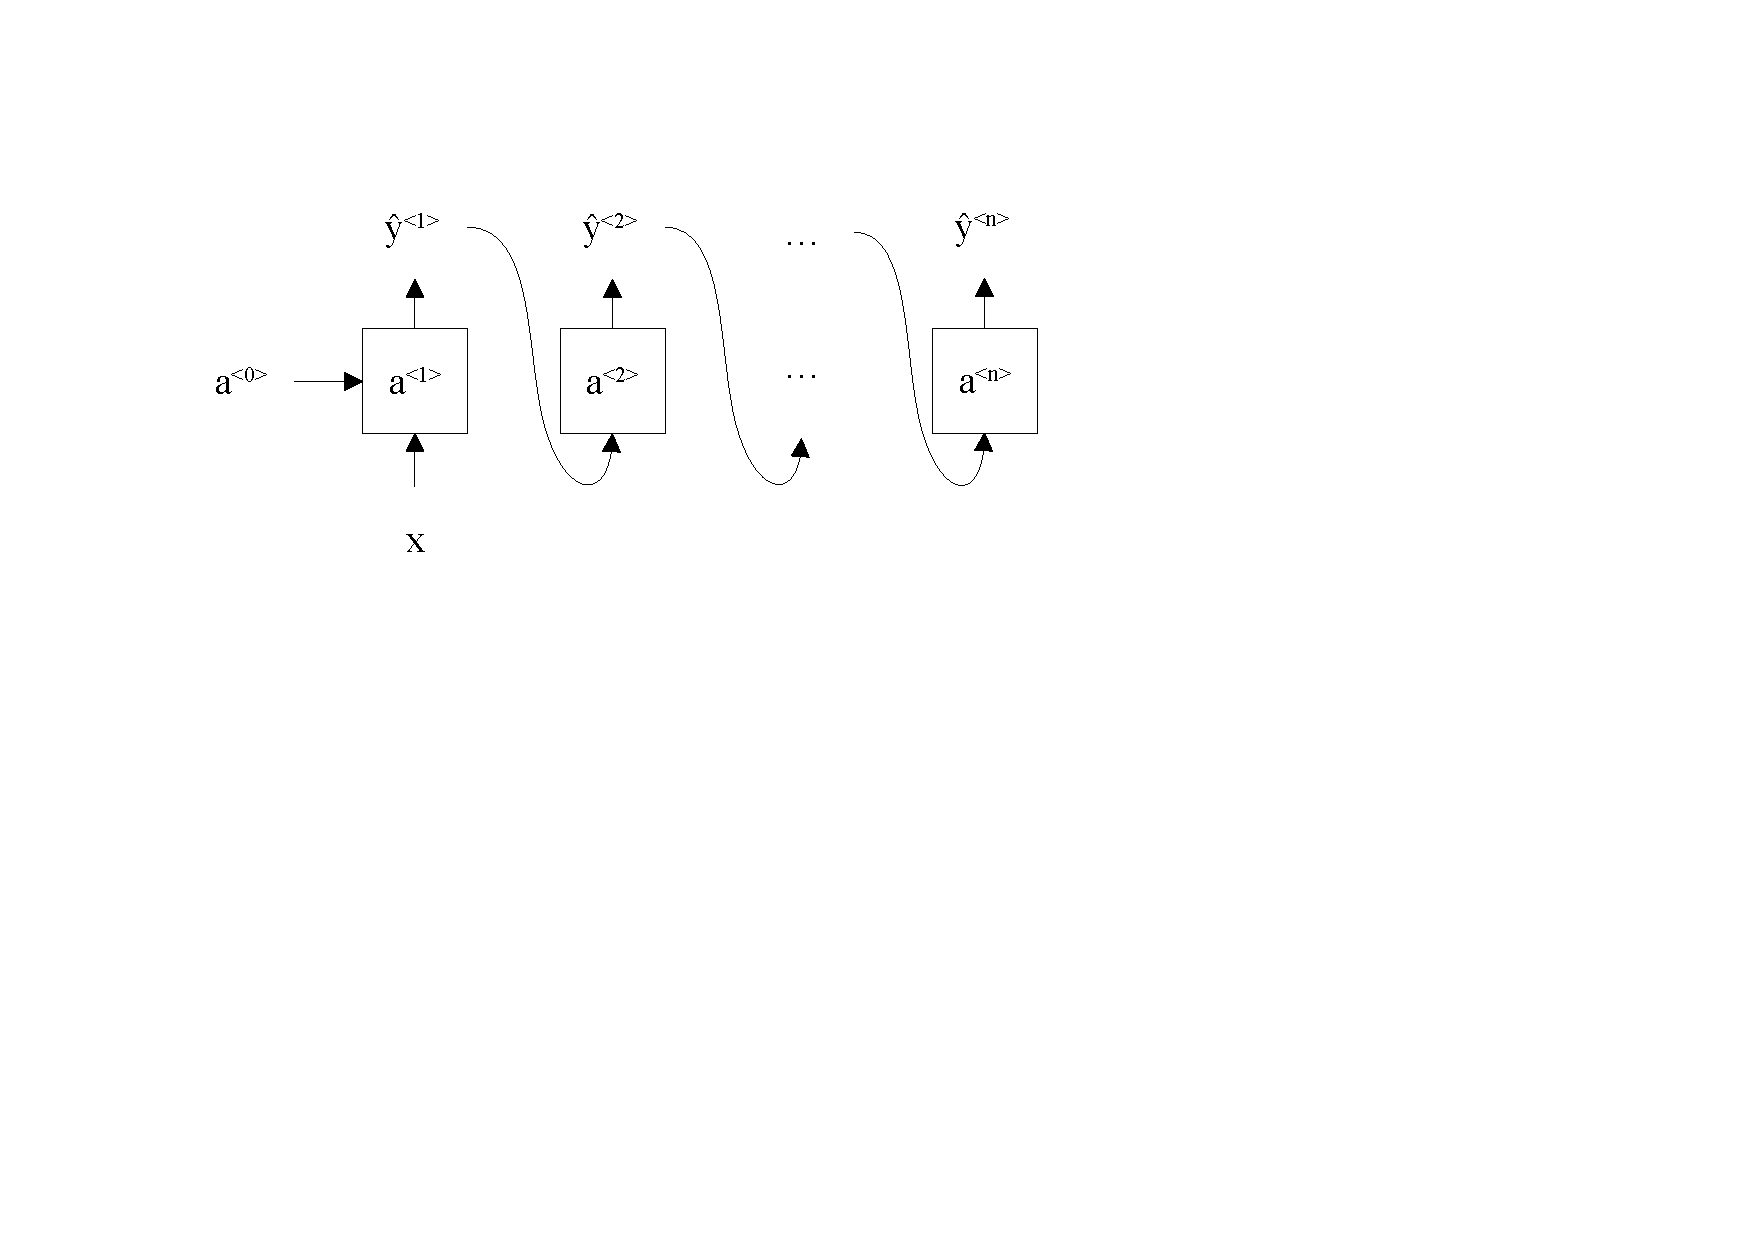
\includegraphics[width=9cm]{chapter07/figure-sec12/one-to-many-rnn.pdf}
    \caption{Mô hình mạng one-to-many RNN}
    \label{fig:one-to-many-rnn}
\end{figure}

\begin{exmp}
\label{exmp:ln-rnn-simple}
với câu “Hôm nay tôi đi học”, ta có mạng RNN như hình \ref{fig:lm-rnn-simple}
\begin{figure}[h!]
    \centering
    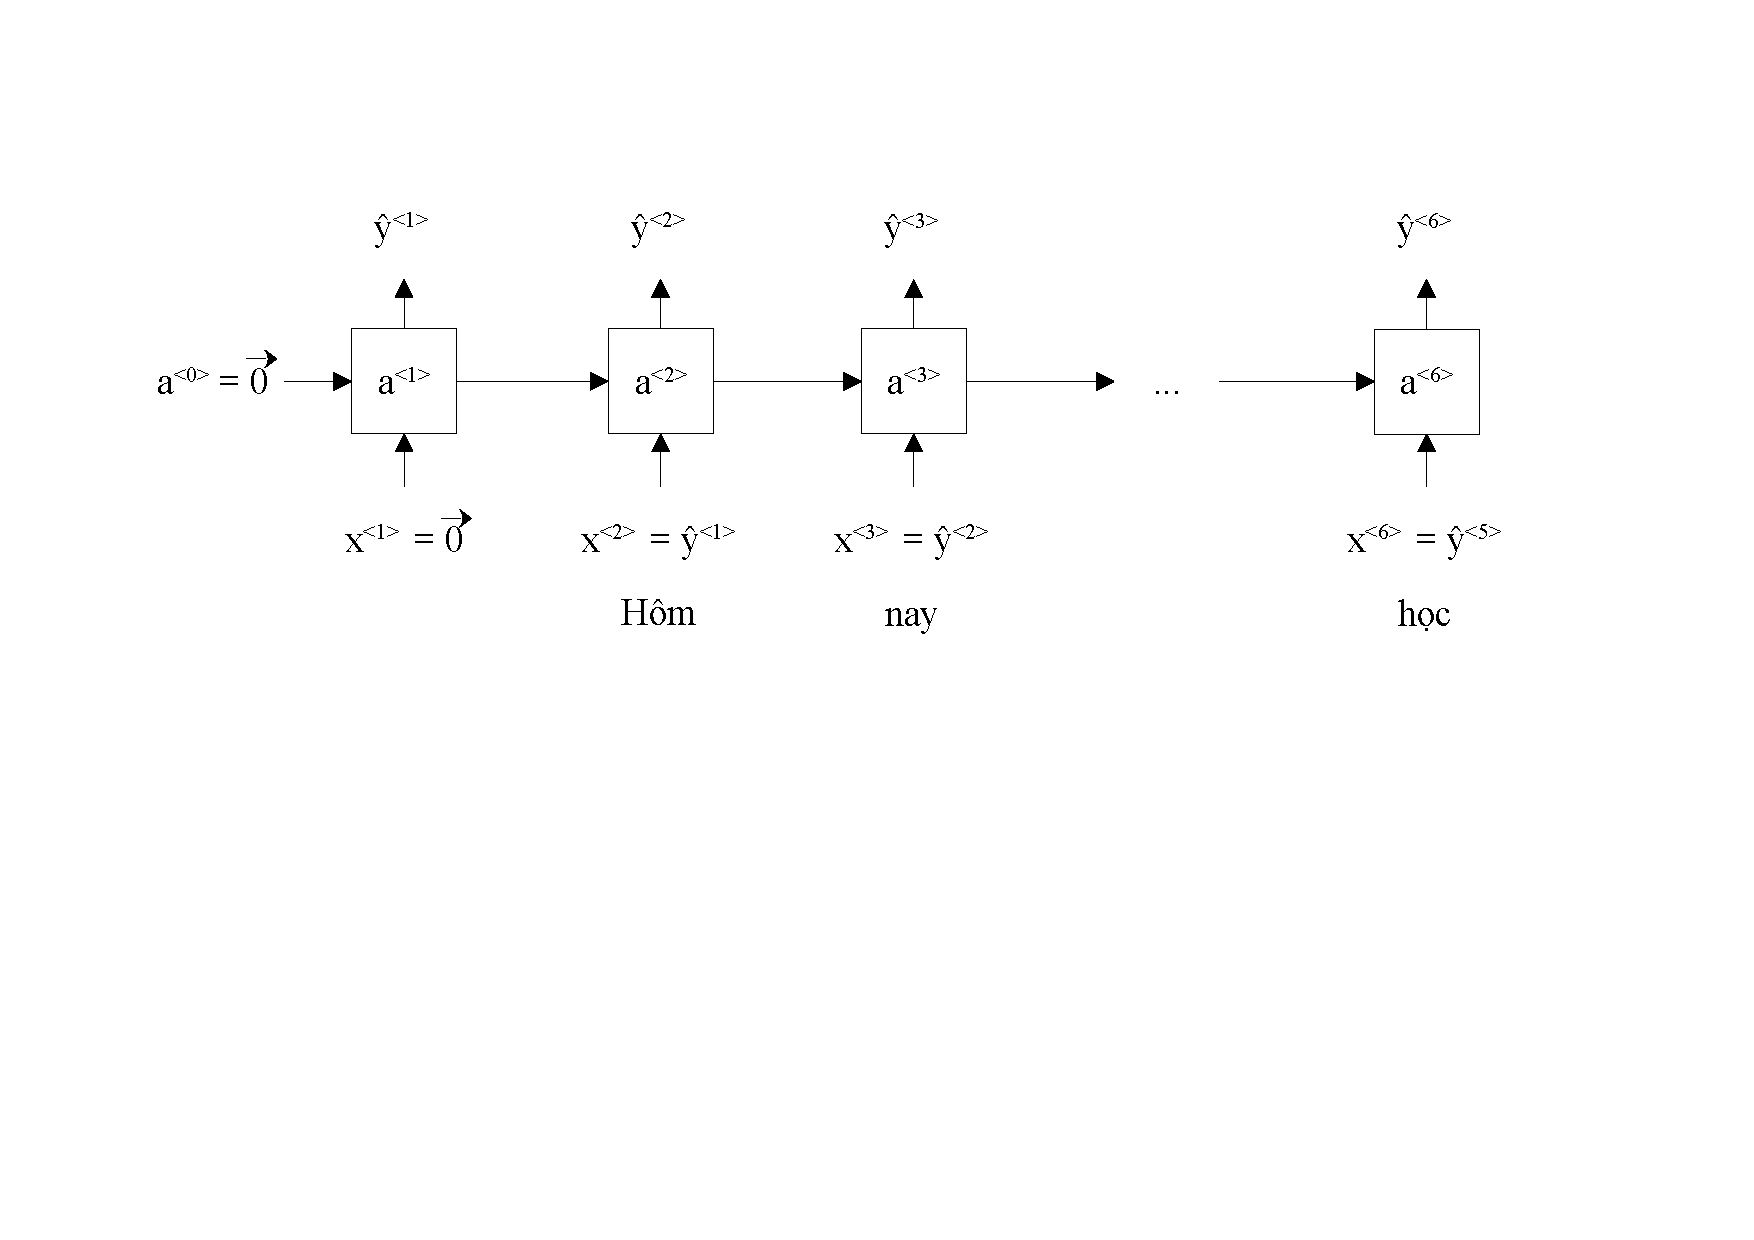
\includegraphics[width=13cm]{chapter07/figure-sec12/lm-rnn-simple.pdf}
    \caption{Mô hình đơn giản thể hiện ý tưởng huấn luyện Language Model với RNN}
    \label{fig:lm-rnn-simple}
\end{figure}
\end{exmp}
Trong ví dụ \ref{exmp:ln-rnn-simple}, ở đầu câu, chúng ta chưa có từ đứng trước, vì thế ta sẽ truyền vào $x^{<1>}$ và $a^{<0>}$ là vector 0 để khởi động cho mạng với ý nghĩa đầu vào là từ “mở đầu câu”, như vậy:

\begin{itemize}
\item $\hat{y}^{<1>}$ là xác suất từ “Hôm” là xuất hiện ở đầu câu $P(\textit{Hôm})$,
% Tương tự:\\
\item $\hat{y}^{<2>}$ là xác suất từ “nay” xuất hiện sau từ “Hôm” ở đầu câu $P(\textit{nay} \mid \textit{Hôm})$,
\item $\hat{y}^{<3>}$ là xác suất từ “tôi” xuất hiện sau “Hôm nay” $P(\textit{tôi} \mid \textit{Hôm nay})$,
\item $\hat{y}^{<4>}$ là xác suất từ “đi” xuất hiện sau “Hôm nay tôi” $P(\textit{đi} \mid$ \textit{Hôm nay tôi}$)$,
\item $\hat{y}^{<5>}$ là xác suất từ “tôi” xuất hiện sau “Hôm nay tôi đi” $P(\textit{học} \mid$ \textit{Hôm nay tôi đi}$)$,
\item $\hat{y}^{<6>}$ là xác suất câu kết thúc tại “Hôm nay tôi đi học” $P(\textit{<EOS>} \mid$ \textit{Hôm nay tôi đi học}$)$, tức xác suất “Hôm nay tôi đi học” là một câu hoàn chỉnh.
\end{itemize}

Ngoài ra, chúng ta có thể tính được xác suất của một câu, một cụm từ nào đó có thể xuất hiện hay không bằng công thức tương tự như ví dụ sau:
\begin{align*}
    P(y^{<1>}, y^{<2>}, y^{<3>}) & = P(y^{<1>})P(y^{<2>} \mid y^{<1>})P(y^{<3>} \mid y^{<1>}, y^{<2>})\\
    & = \hat{y}^{<1>}\hat{y}^{<2>}\hat{y}^{<3>}
\end{align*}

Với mô hình huấn luyện như trên, nếu ta sử dụng hàm kích hoạt softmax và tập dữ liệu huấn luyện là tập từ vựng trong từ điển thì kết quả đầu ra ở mỗi lần lặp là xác suất xuất hiện của mỗi từ trong từ điển nếu biết xác suất hiện của các từ đó trước đó trong câu.

\subsection{Huấn luyện Language Model với RNN}
Tương tự với các bài toán xử lí ngôn ngữ tự nhiên khác, trước khi huấn luyện một language model, chúng ta cần có bước tiền xử lí. Ở bước này chúng ta sẽ vec-tơ hóa các từ trong từ điển bằng các phương pháp đã trình bày ở các chương trước như one-hot vector, hay các kỹ thuật word embedding khác,...\par
Lưu ý, khi vec-tơ hóa sẽ gặp các trường hợp một từ là số, tên riêng, các từ ít gặp, hoặc các từ, vị trí đặc biệt có ý nghĩa mà ta muốn sử dụng cho ứng dụng của mình. Đối với các từ này, ta sẽ thay thế bằng các token tổng quát. Ví dụ:
\begin{itemize}
\setlength\itemsep{-0.5em}
\item số thay bằng <NUM>.
\item các từ ít gặp thay bằng <UNK>.
\item thêm các token đặc biệt như <EOS> - token kết thúc câu.
\end{itemize}\par
Việc dùng các token này giúp mô hình tránh được việc quá khớp với các từ khác nhau có cùng ý nghĩa hoặc vai trò trong câu như các con số, các tên riêng,… hay giúp mô hình nhận biết được một câu hoàn chỉnh bằng token <EOS>. Sau khi thực hiện tiền xử lí xong, ta sẽ dùng mạng RNN để huấn luyện language model. Cụ thể, ta cùng khảo sát ví dụ \ref{exmp:ln-rnn-detail}.\par

\begin{exmp}
\label{exmp:ln-rnn-detail}
Huấn luyện Language Model với tài liệu:\\ "Hôm nay tôi đi học. Ngày mai tôi cũng đi học."\par
Giả sử corpus chỉ gồm các từ trong tài liệu này, sử dụng one-hot vector để biểu diễn các từ trong corpus, ta sẽ có mỗi từ là một véc-tơ 1x8. Input $x^{<0>}$ sẽ là một véc-tơ 0 với số chiều phụ thuộc vào corpus, trong trường hợp này là 1x8.
Trạng thái bắt đầu $a^{<0>}$ là một vec-tơ 0 với số chiều tùy thuộc vào thiết kế của chúng ta, ở đây chọn vec-tơ 1x5.\par

\begin{figure}[h!]
    \centering
    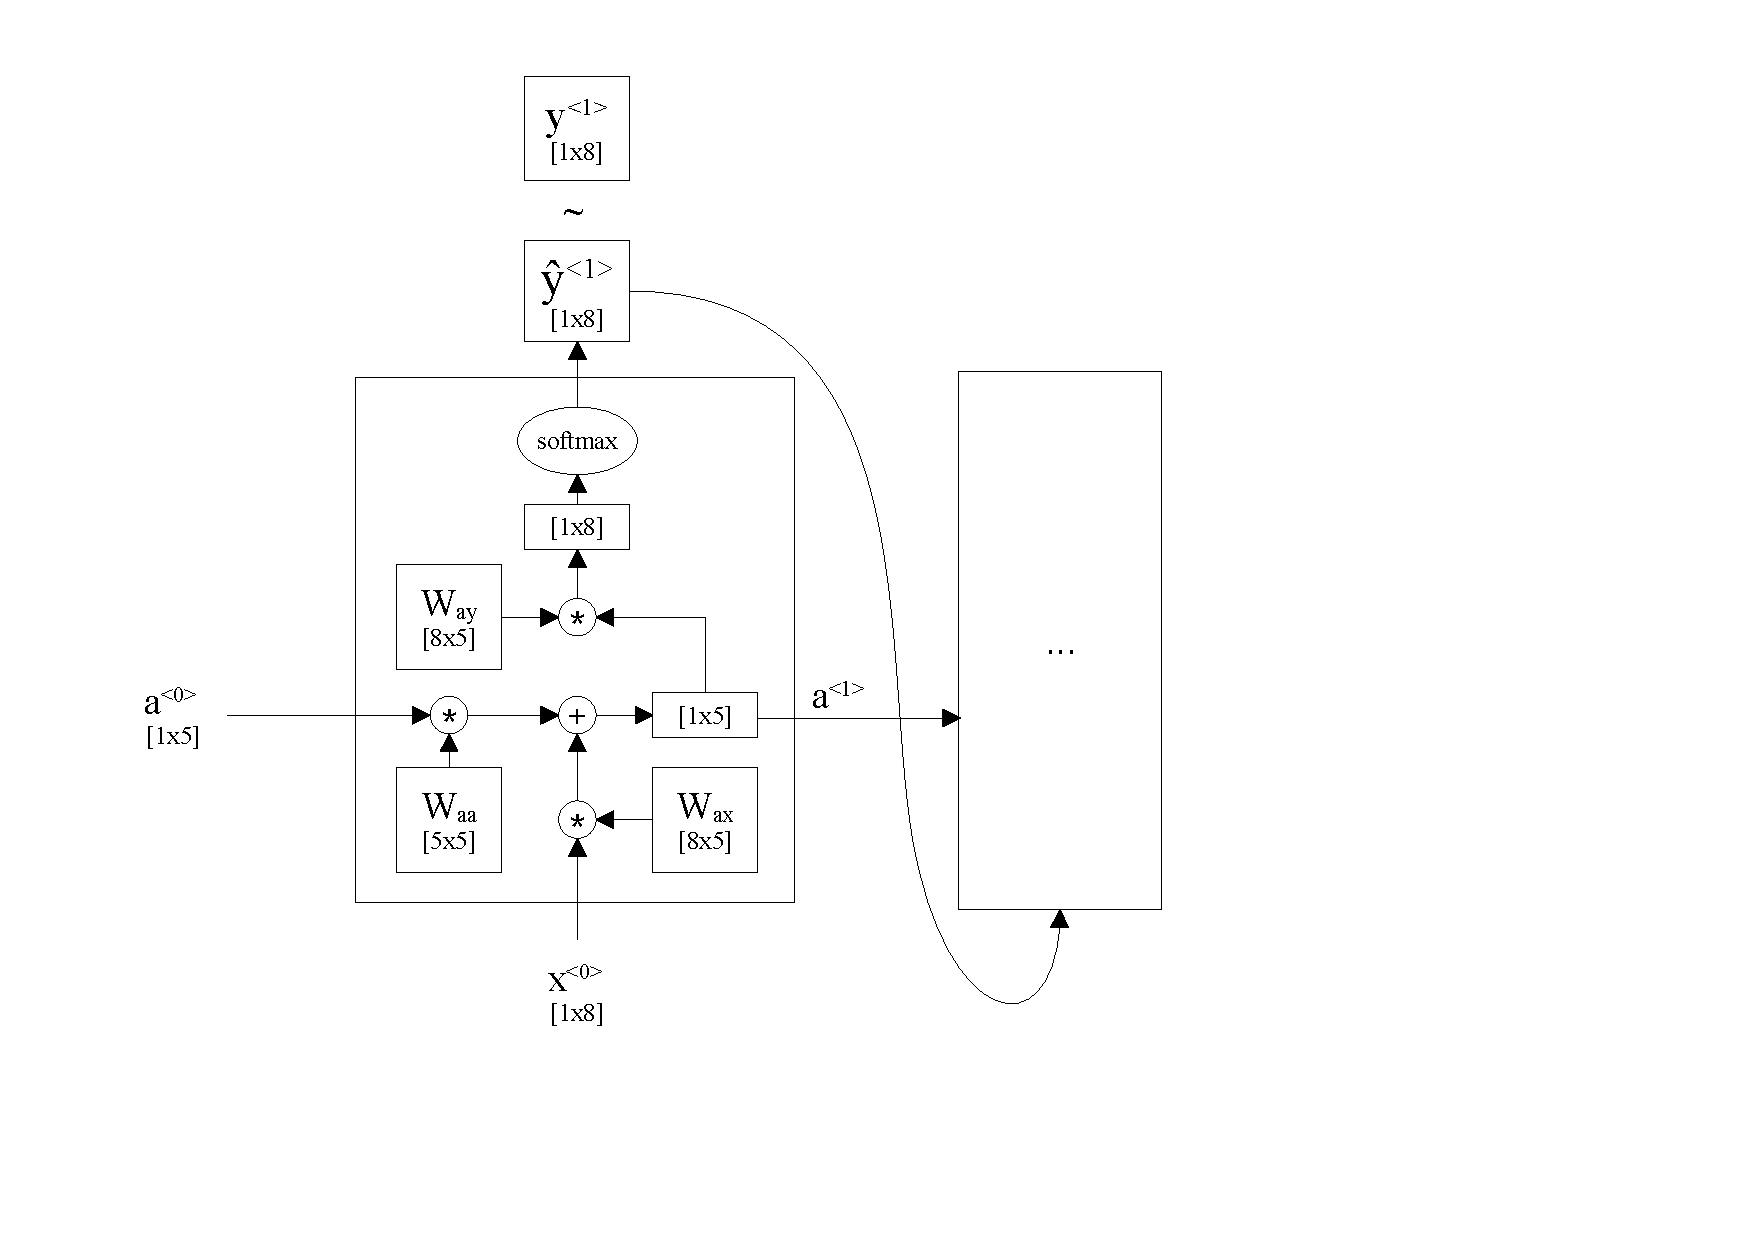
\includegraphics[width=13cm]{chapter07/figure-sec12/lm-rnn-detail.pdf}
    \caption{Minh họa ví dụ \ref{exmp:ln-rnn-detail}, huấn luyện Language Model với RNN}
    \label{fig:lm-rnn-detail}
\end{figure}

Khi đó, $W_{aa}$ là một ma trận 5x5, $W_{ax}$ là một ma trận 8x5. Đầu ra của phép tính $W_{aa}a^{<i>} + W_{ax}x^{<i>}$ là một vec-tơ 1x5, trong khi đó ta cần kết quả $\hat{y}$ là một vec-tơ 1x8 để so sánh được với các véc-tơ trong corpus. Do đó, $W_{ay}$ sẽ là ma trận 5x8.\par
Ta chọn hàm kích hoạt là hàm softmax để chuyển kết quả về khoảng [0, 1], tức thành xác suất rơi vào các từ trong corpus đang được biểu diễn dưới dạng one-hot. Sau đó sử dụng các phương pháp tối ưu hàm mất mát của softmax để cập nhật các ma trận trọng số.
\end{exmp}
Hàm mất mát tại thời điểm $t$:
$$
\mathcal{L}(\hat{y}^{<t>}, y^{<t>}) = - \sum\limits_{i}{y_i^{<t>}\log{\hat{y}_i^{<t>}}}
$$\par
Tổng mất mát:
$$
\mathcal{L} = \sum\limits_{t}{\mathcal{L}(\hat{y}^{<t>}, y^{<t>})}
$$

Theo mô hình RNN trên, mất mát sẽ được tính ở cuối corpus để cập nhật trọng số. Trọng số chỉ được học hiệu quả khi corpus lớn, có thể lên đến vài tỉ từ. Việc này gây nhiều khó khăn do giới hạn của bộ nhớ máy tính. Giải pháp cho vấn đề này là ta sẽ cắt theo một số lượng từ nhất định để tính mất mát và cập nhật trọng số, không nhất thiết phải là tại vị trí kết thúc câu.
